%	CHAP Docker%----------------------------------------------------------------------------------------

\chapterimage{blue-chapter-head_4-reduced.pdf} % Chapter heading image

\chapter{Docker Integration}\label{chap:DockerIntegration}
The integration with Docker helps with the reprducibility of your analyses. Installing packages with R does not make it possible to specific exactly the version of the package that you need for an analysis. While it is possible to always install the latest version of a package, the behavior of some packages will change over time. For this reason, it is useful to build snapshots of the R packages used during analysis and report the version number of the snapshot. 

\section{Pre-requisites}
You will need a working docker installation on your machine before you can run MetaR analyses with Docker.
\subsection{Mac OS}
\begin{SCfigure}
  \centering
  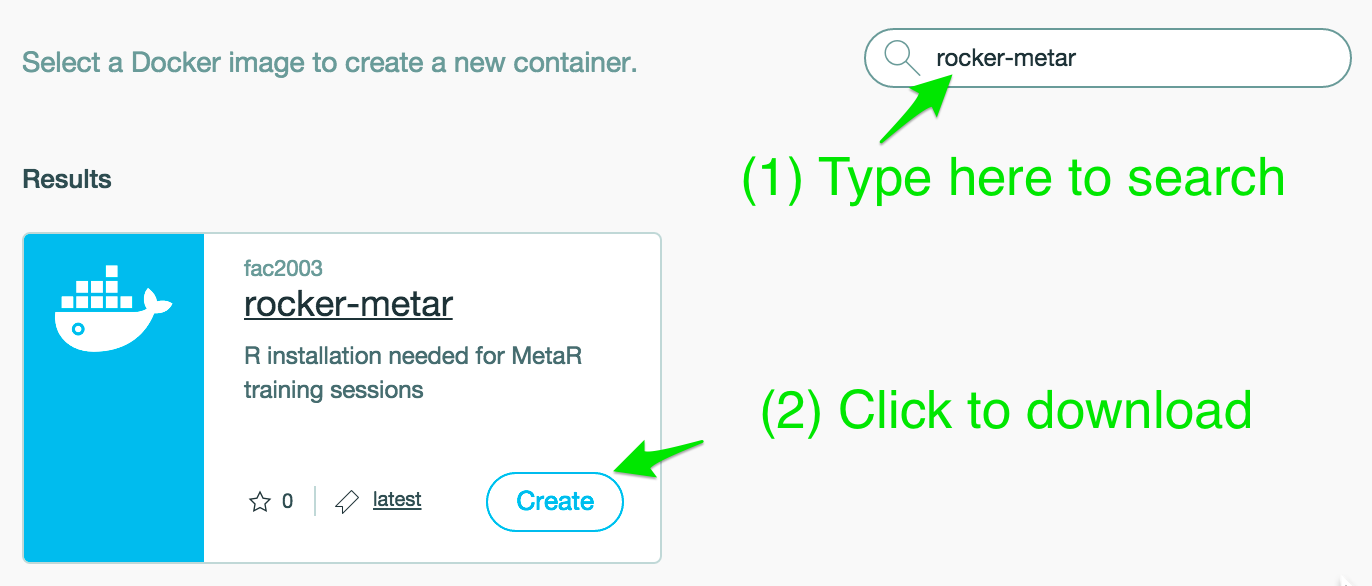
\includegraphics[width=\figWidthNarrow]{figures/Rocker-MetaR-Image.png}
\caption[Download the MetaR Docker Image.]{\textbf{Download the MetaR Docker Image.} Follow steps steps to locate the MetaR Docker image.}
\label{fig:RockerMetaRImage}
\end{SCfigure}

Mac users will find it convenient to download and install Kitematic (\url{https://kitematic.com/}). 
 After you unzip Kitematic, move the application to /Applications and start it. Wait until the virtual machine downloads and starts. When kitematic is ready, use the search box to locate the \texttt{rocker-metar} image (see Figure~\ref{fig:RockerMetaRImage} for instructions). 


\subsection{Other Platforms}
 Other users should refer to documented installation steps for their platform (see \url{http://docs.docker.com/installation/}).

\section{Configuring Docker}\index{Docker}
Docker integration can be configured using the MPS Preferences.  Open Preferences (Setting on Windows) and locate the Docker configuration (use the search box with the docker keyword). You will be presented with the following dialog shown in Figure~\ref{fig:DockerPreferencesDialog}.

\begin{figure}[h!tbp]
  \centering
  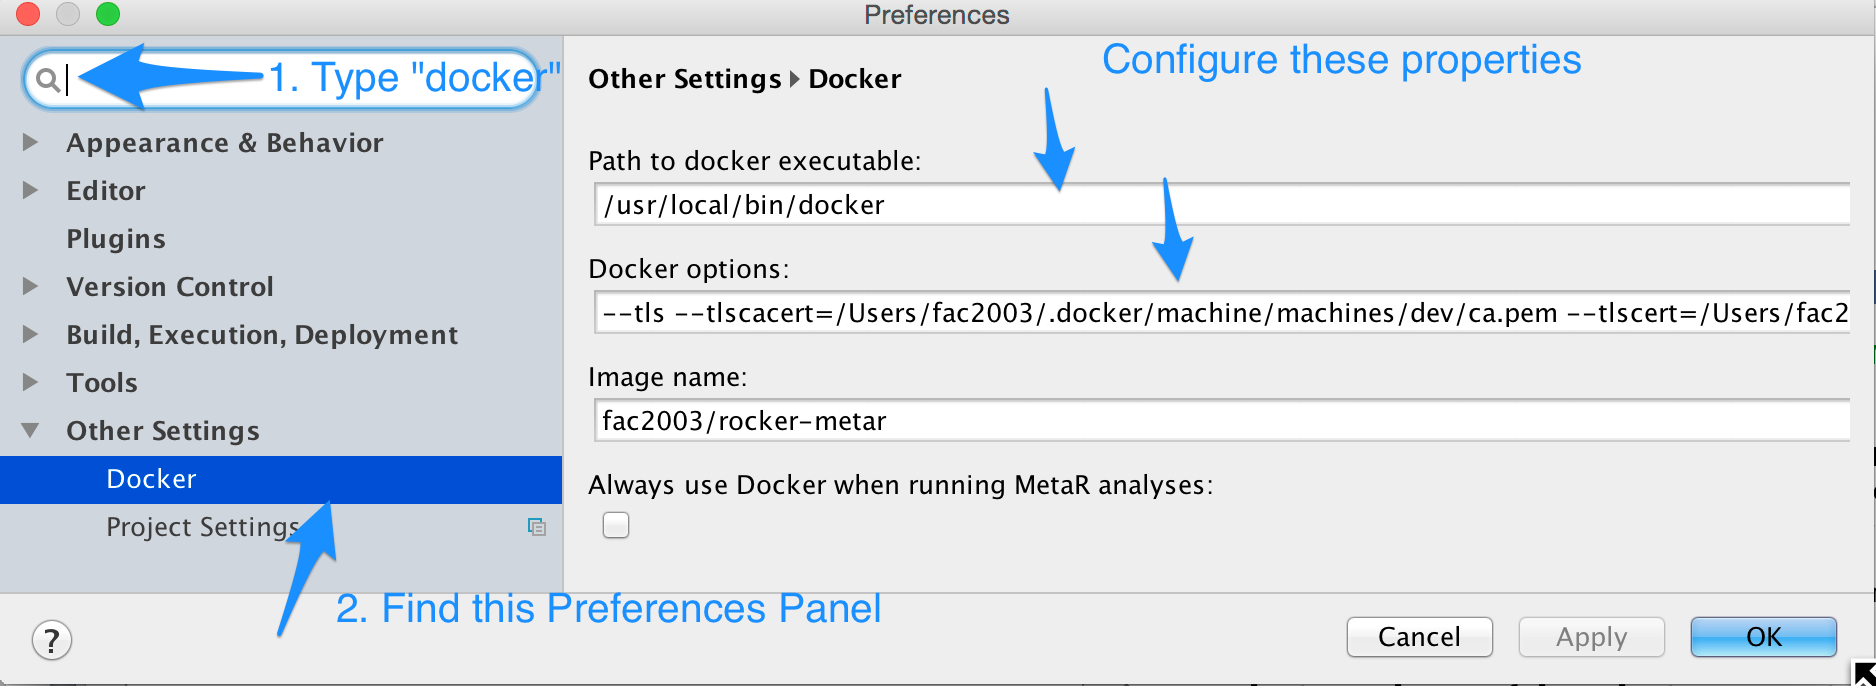
\includegraphics[width=\figWidthWide]{figures/DockerPreferencesDialog.png}
\caption[Docker Configuration Dialog.]{\textbf{Docker Configuration Dialog.} This dialog is available under MPS Preferences/Settings.}
\label{fig:DockerPreferencesDialog}
\end{figure}

\paragraph{path to docker executable}
This field must provide a path to a valid docker executable. On linux, try \texttt{which docker} in the shell. On Mac, if you installed Kitematic\index{Kitematic}, open the application and start the terminal with the \menu{File>Open Docker Command}\allowbreak\menu{Line Terminal Window}. In the window, type \texttt{which docker} and copy the location to the field. 

\paragraph{docker options}
These are the options necessary to connect to the docker server. On Mac, if you installed Kitematic, open the application and start the terminal with the \menu{File>Open Docker Command}\allowbreak\menu{Line Terminal Window}. In the window, type \texttt{echo `docker-machine config`} and copy the line printed to the field. 

\paragraph{image name}
This is the name of the docker image that you wish to use with MetaR. Keep the default, or enter a customized image name here. Customizing the image is useful if you need to install additional packages than the ones we use during our training sessions. If you create a new image, make sure you use \texttt{fac2003/rocker-metar} in the FROM field. Images that do not build on \texttt{fac2003/rocker-metar} are not supported at this time.

\begin{remark}
Note that you can specify an image tag/version number. Append a colon (:) and the tag after the image name. For instance, use \texttt{fac2003/rocker-metar:1.3.1} to run the \texttt{rocker-metar} image packaged with MetaR 1.3.1.  
\end{remark}

\begin{remark}
Note that specifying a tag is a good idea if you need to reproduce exactly an analysis in the future. Omitting the tag will always get the latest version of the image, which may change over time.  
\end{remark}

\paragraph{always use docker}
This checkbox can be use to force the use of Docker by default when running an Analysis. This is convenient if you know that you configuration is correct and want to run all analyses with docker. 

\section{Running with Docker}
When docker is successfully configured, you can specify to use the docker image when running a MetaR analysis. See instructions in Figure~\ref{fig:RunWithDocker} to see how to configure running insider a Docker container.

\begin{SCfigure}
  \centering
  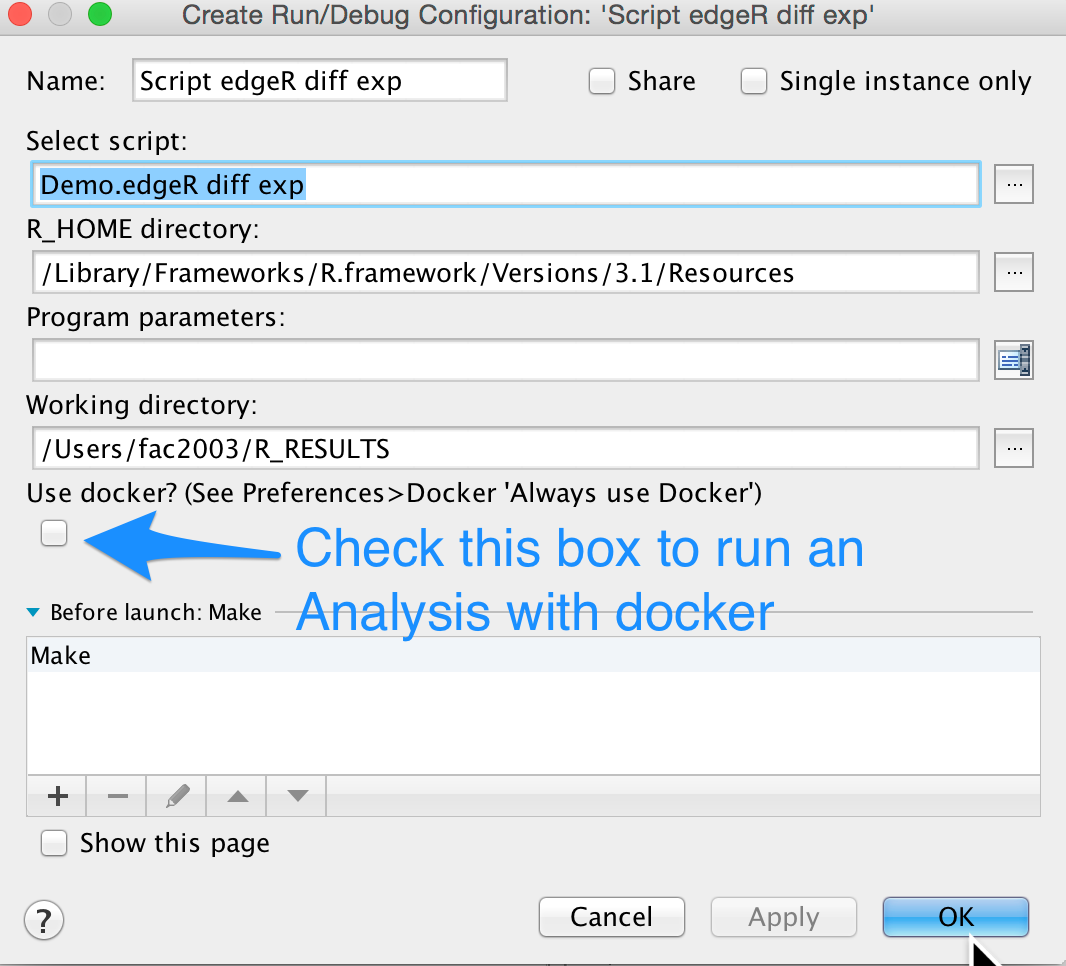
\includegraphics[width=\figWidthNarrow]{figures/CheckThisBoxToRunWithDocker.png}
\caption[Run With Docker.]{\textbf{Run With Docker.} Right-click on an Analysis and do \menu{Create <analysis name>}. You will be presented with the Run Configuration customization dialog. Check the box to run with docker. Disable the check-box to run directly against the R installation on your computer (this behavior was the default prior for MetaR 1.3-).  }
\label{fig:RunWithDocker}
\end{SCfigure}


